% Options for packages loaded elsewhere
\PassOptionsToPackage{unicode}{hyperref}
\PassOptionsToPackage{hyphens}{url}
\PassOptionsToPackage{dvipsnames,svgnames,x11names}{xcolor}
%
\documentclass[
  letterpaper,
  DIV=11,
  numbers=noendperiod]{scrartcl}

\usepackage{amsmath,amssymb}
\usepackage{lmodern}
\usepackage{iftex}
\ifPDFTeX
  \usepackage[T1]{fontenc}
  \usepackage[utf8]{inputenc}
  \usepackage{textcomp} % provide euro and other symbols
\else % if luatex or xetex
  \usepackage{unicode-math}
  \defaultfontfeatures{Scale=MatchLowercase}
  \defaultfontfeatures[\rmfamily]{Ligatures=TeX,Scale=1}
\fi
% Use upquote if available, for straight quotes in verbatim environments
\IfFileExists{upquote.sty}{\usepackage{upquote}}{}
\IfFileExists{microtype.sty}{% use microtype if available
  \usepackage[]{microtype}
  \UseMicrotypeSet[protrusion]{basicmath} % disable protrusion for tt fonts
}{}
\makeatletter
\@ifundefined{KOMAClassName}{% if non-KOMA class
  \IfFileExists{parskip.sty}{%
    \usepackage{parskip}
  }{% else
    \setlength{\parindent}{0pt}
    \setlength{\parskip}{6pt plus 2pt minus 1pt}}
}{% if KOMA class
  \KOMAoptions{parskip=half}}
\makeatother
\usepackage{xcolor}
\setlength{\emergencystretch}{3em} % prevent overfull lines
\setcounter{secnumdepth}{-\maxdimen} % remove section numbering
% Make \paragraph and \subparagraph free-standing
\ifx\paragraph\undefined\else
  \let\oldparagraph\paragraph
  \renewcommand{\paragraph}[1]{\oldparagraph{#1}\mbox{}}
\fi
\ifx\subparagraph\undefined\else
  \let\oldsubparagraph\subparagraph
  \renewcommand{\subparagraph}[1]{\oldsubparagraph{#1}\mbox{}}
\fi


\providecommand{\tightlist}{%
  \setlength{\itemsep}{0pt}\setlength{\parskip}{0pt}}\usepackage{longtable,booktabs,array}
\usepackage{calc} % for calculating minipage widths
% Correct order of tables after \paragraph or \subparagraph
\usepackage{etoolbox}
\makeatletter
\patchcmd\longtable{\par}{\if@noskipsec\mbox{}\fi\par}{}{}
\makeatother
% Allow footnotes in longtable head/foot
\IfFileExists{footnotehyper.sty}{\usepackage{footnotehyper}}{\usepackage{footnote}}
\makesavenoteenv{longtable}
\usepackage{graphicx}
\makeatletter
\def\maxwidth{\ifdim\Gin@nat@width>\linewidth\linewidth\else\Gin@nat@width\fi}
\def\maxheight{\ifdim\Gin@nat@height>\textheight\textheight\else\Gin@nat@height\fi}
\makeatother
% Scale images if necessary, so that they will not overflow the page
% margins by default, and it is still possible to overwrite the defaults
% using explicit options in \includegraphics[width, height, ...]{}
\setkeys{Gin}{width=\maxwidth,height=\maxheight,keepaspectratio}
% Set default figure placement to htbp
\makeatletter
\def\fps@figure{htbp}
\makeatother

\KOMAoption{captions}{tableheading}
\makeatletter
\makeatother
\makeatletter
\makeatother
\makeatletter
\@ifpackageloaded{caption}{}{\usepackage{caption}}
\AtBeginDocument{%
\ifdefined\contentsname
  \renewcommand*\contentsname{Table of contents}
\else
  \newcommand\contentsname{Table of contents}
\fi
\ifdefined\listfigurename
  \renewcommand*\listfigurename{List of Figures}
\else
  \newcommand\listfigurename{List of Figures}
\fi
\ifdefined\listtablename
  \renewcommand*\listtablename{List of Tables}
\else
  \newcommand\listtablename{List of Tables}
\fi
\ifdefined\figurename
  \renewcommand*\figurename{Figure}
\else
  \newcommand\figurename{Figure}
\fi
\ifdefined\tablename
  \renewcommand*\tablename{Table}
\else
  \newcommand\tablename{Table}
\fi
}
\@ifpackageloaded{float}{}{\usepackage{float}}
\floatstyle{ruled}
\@ifundefined{c@chapter}{\newfloat{codelisting}{h}{lop}}{\newfloat{codelisting}{h}{lop}[chapter]}
\floatname{codelisting}{Listing}
\newcommand*\listoflistings{\listof{codelisting}{List of Listings}}
\makeatother
\makeatletter
\@ifpackageloaded{caption}{}{\usepackage{caption}}
\@ifpackageloaded{subcaption}{}{\usepackage{subcaption}}
\makeatother
\makeatletter
\@ifpackageloaded{tcolorbox}{}{\usepackage[many]{tcolorbox}}
\makeatother
\makeatletter
\@ifundefined{shadecolor}{\definecolor{shadecolor}{rgb}{.97, .97, .97}}
\makeatother
\makeatletter
\makeatother
\ifLuaTeX
  \usepackage{selnolig}  % disable illegal ligatures
\fi
\IfFileExists{bookmark.sty}{\usepackage{bookmark}}{\usepackage{hyperref}}
\IfFileExists{xurl.sty}{\usepackage{xurl}}{} % add URL line breaks if available
\urlstyle{same} % disable monospaced font for URLs
\hypersetup{
  pdftitle={MF\_01\_Modelfree\_Analysis},
  pdfauthor={Julius Kricheldorff},
  colorlinks=true,
  linkcolor={blue},
  filecolor={Maroon},
  citecolor={Blue},
  urlcolor={Blue},
  pdfcreator={LaTeX via pandoc}}

\title{MF\_01\_Modelfree\_Analysis}
\author{Julius Kricheldorff}
\date{}

\begin{document}
\maketitle
\ifdefined\Shaded\renewenvironment{Shaded}{\begin{tcolorbox}[interior hidden, frame hidden, borderline west={3pt}{0pt}{shadecolor}, sharp corners, enhanced, breakable, boxrule=0pt]}{\end{tcolorbox}}\fi

\hypertarget{load-all-data-files-and-set-working-environment}{%
\subsection{Load all data files and set working
environment}\label{load-all-data-files-and-set-working-environment}}

In this chunk we load and set up the data.

\hypertarget{plot-reaction-times-by-task-and-stimulation-condition}{%
\subsection{Plot Reaction Times by Task and Stimulation
condition}\label{plot-reaction-times-by-task-and-stimulation-condition}}

First we plot the reaction times for each task, only for the correct
trials

\hypertarget{reaction-time-simple-reaction-time-task}{%
\subsubsection{Reaction Time Simple Reaction Time
Task}\label{reaction-time-simple-reaction-time-task}}

First we plot the reaction times for the simple stimulus response task.
We see a little more variability in the non-therapeutic stimulation
conditions, but arguably no difference in RT.

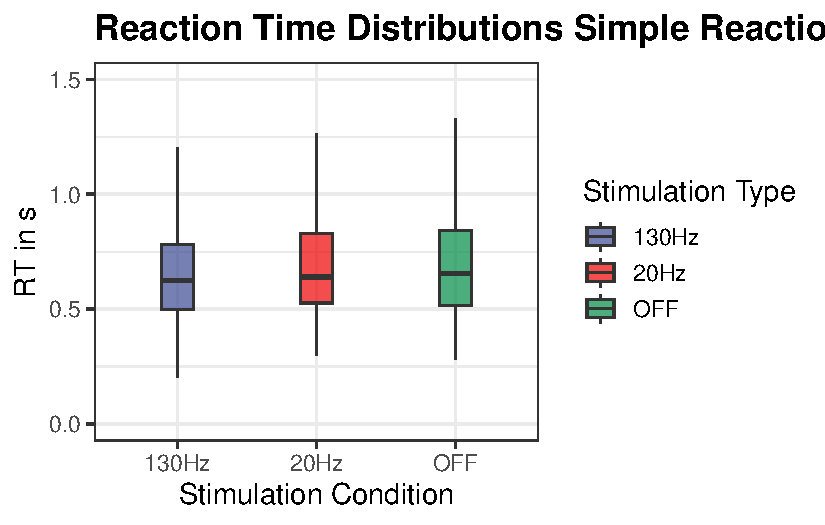
\includegraphics{MF_01_Modelfree_Analysis_files/figure-pdf/unnamed-chunk-2-1.pdf}

\hypertarget{reaction-time-flanker-task}{%
\subsubsection{Reaction Time Flanker
Task}\label{reaction-time-flanker-task}}

Looking at the flanker data, there does seem to be some kind of main
effect, with faster RTs in the 130Hz condition, but nothing else beside
that.

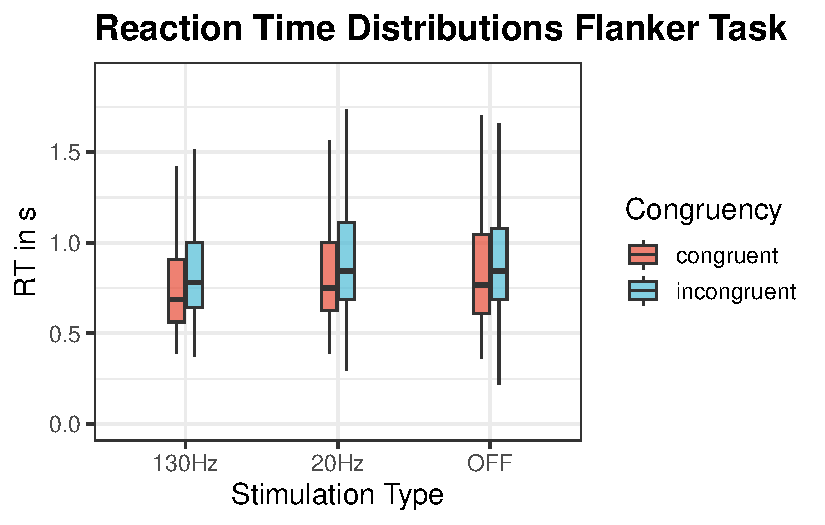
\includegraphics{MF_01_Modelfree_Analysis_files/figure-pdf/unnamed-chunk-3-1.pdf}

\hypertarget{reaction-time-go-nogo-task}{%
\subsubsection{Reaction Time Go-NoGo
Task}\label{reaction-time-go-nogo-task}}

Arguably, slightly slower performance on the NoGo - Go trials for the
20Hz participants?

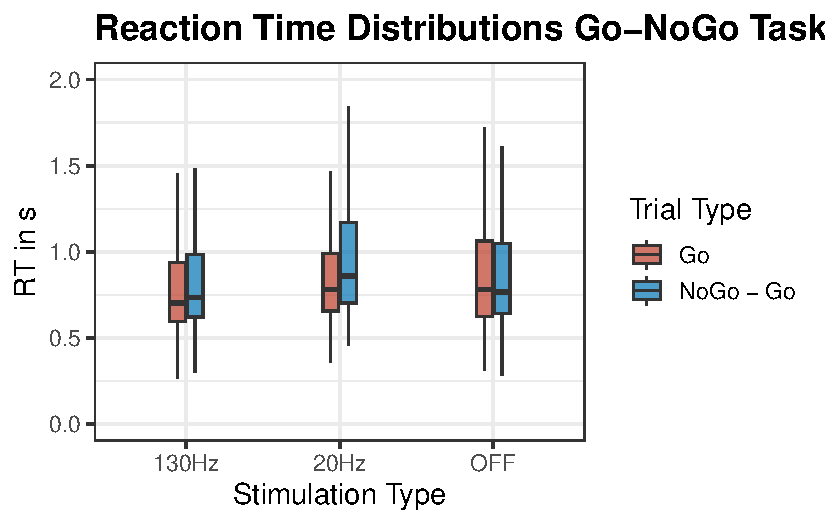
\includegraphics{MF_01_Modelfree_Analysis_files/figure-pdf/unnamed-chunk-4-1.pdf}

\hypertarget{reaction-time-stop-signal-task}{%
\subsubsection{Reaction Time Stop-Signal
Task}\label{reaction-time-stop-signal-task}}

Arguably much more variability on the Stop trials in the 130Hz
participants.

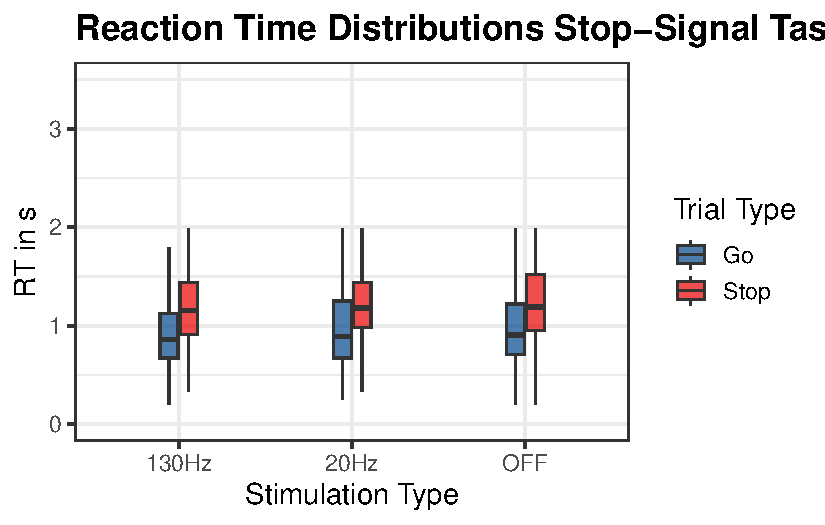
\includegraphics{MF_01_Modelfree_Analysis_files/figure-pdf/unnamed-chunk-5-1.pdf}

Because this is not actually what we are after, we will also claculate
the Stop-Signal reaction time

\begin{verbatim}
`summarise()` has grouped output by 'Part_nr'. You can override using the
`.groups` argument.
`summarise()` has grouped output by 'Part_nr'. You can override using the
`.groups` argument.
Adding missing grouping variables: `Part_nr`
New names:
\end{verbatim}

\begin{verbatim}
# A tibble: 3 x 2
  Stim_verb  mean
  <chr>     <dbl>
1 130Hz     0.611
2 20Hz      0.695
3 OFF       0.687
\end{verbatim}

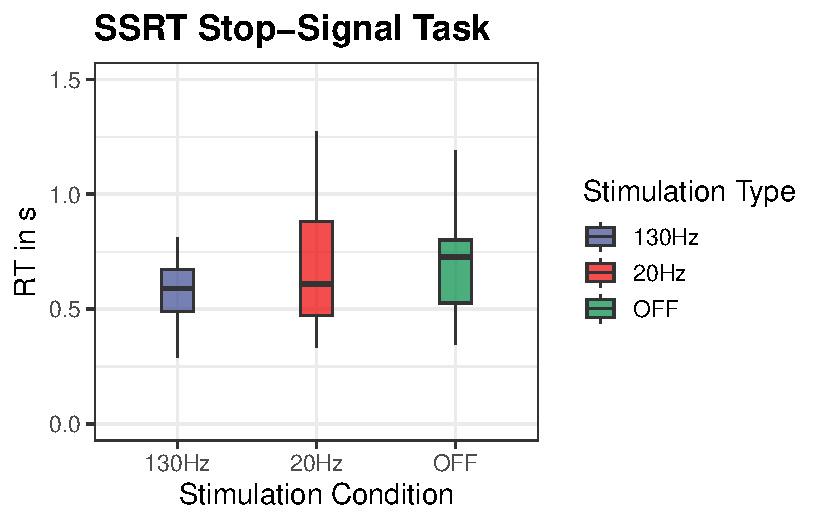
\includegraphics{MF_01_Modelfree_Analysis_files/figure-pdf/unnamed-chunk-6-1.pdf}

\hypertarget{plot-errors-by-task-and-stimulation-condition}{%
\subsection{Plot Errors by Task and Stimulation
condition}\label{plot-errors-by-task-and-stimulation-condition}}

\hypertarget{errors-simple-reaction-time-task}{%
\subsubsection{Errors Simple Reaction Time
Task}\label{errors-simple-reaction-time-task}}

We definitely see fewer error trials in the 20Hz condition here compared
to the 130Hz condition

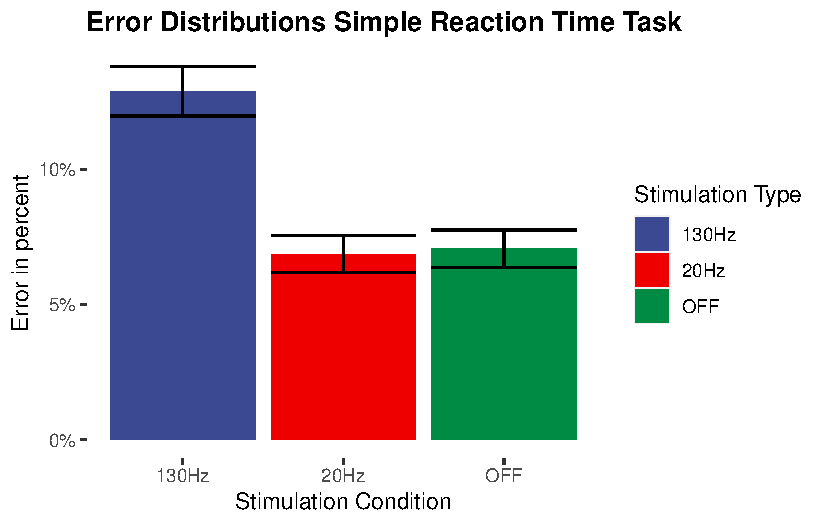
\includegraphics{MF_01_Modelfree_Analysis_files/figure-pdf/unnamed-chunk-7-1.pdf}

\hypertarget{errors-flanker-task}{%
\subsubsection{Errors Flanker Task}\label{errors-flanker-task}}

We definitely see improvements across the board in the 20 Hz data here

\begin{verbatim}
`summarise()` has grouped output by 'Stim_verb'. You can override using the
`.groups` argument.
\end{verbatim}

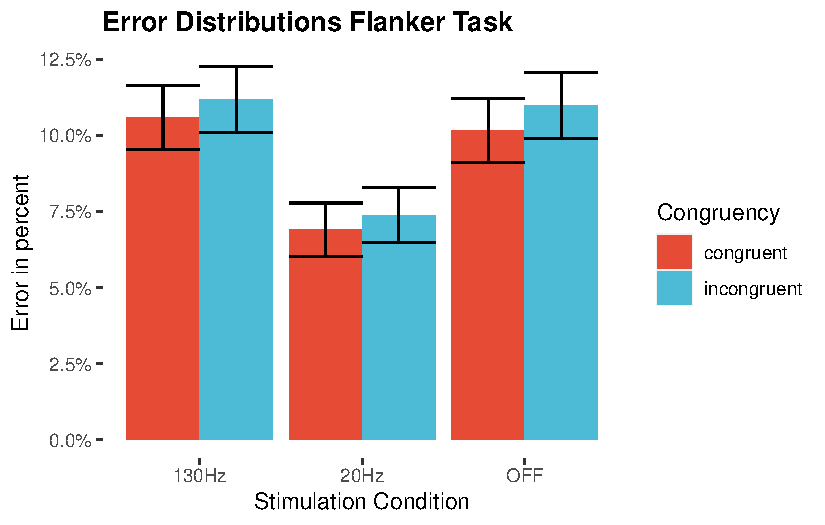
\includegraphics{MF_01_Modelfree_Analysis_files/figure-pdf/unnamed-chunk-8-1.pdf}

\hypertarget{errors-go-nogo-task}{%
\subsubsection{Errors Go-NoGo Task}\label{errors-go-nogo-task}}

Across the board improvements in the Go-NoGo task

\begin{verbatim}
`summarise()` has grouped output by 'Stim_verb'. You can override using the
`.groups` argument.
\end{verbatim}

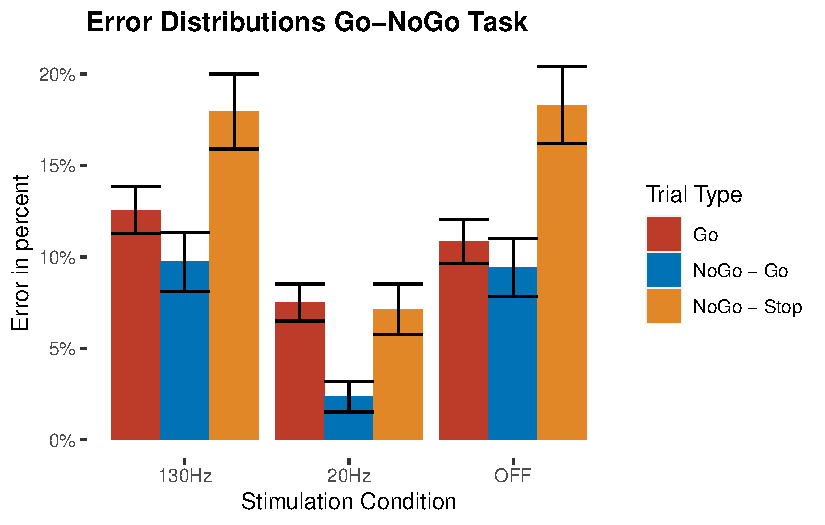
\includegraphics{MF_01_Modelfree_Analysis_files/figure-pdf/unnamed-chunk-9-1.pdf}

\hypertarget{errors-stop-signal-task}{%
\subsubsection{Errors Stop-Signal Task}\label{errors-stop-signal-task}}

Slightly better performance on the Go trials in the 20Hz condition as
compared to the 130Hz conditions

\begin{verbatim}
`summarise()` has grouped output by 'Stim_verb'. You can override using the
`.groups` argument.
\end{verbatim}

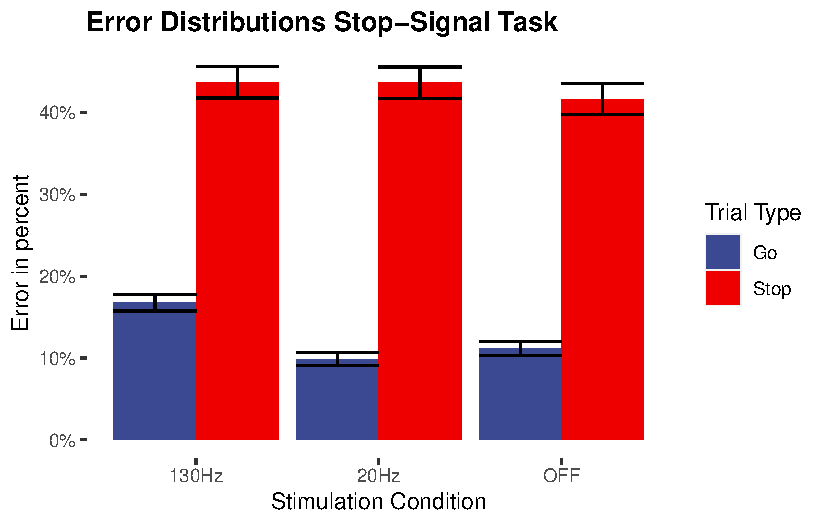
\includegraphics{MF_01_Modelfree_Analysis_files/figure-pdf/unnamed-chunk-10-1.pdf}

\hypertarget{delta-plots}{%
\subsection{Delta Plots}\label{delta-plots}}

First let us generate the data for this

\begin{verbatim}
`summarise()` has grouped output by 'Stim_verb'. You can override using the
`.groups` argument.
`summarise()` has grouped output by 'Stim_verb', 'Congruency'. You can override
using the `.groups` argument.
`summarise()` has grouped output by 'Stim_verb', 'GoNoGo'. You can override
using the `.groups` argument.
`summarise()` has grouped output by 'Stim_verb', 'StopTrl'. You can override
using the `.groups` argument.
\end{verbatim}

\hypertarget{delta-plot-simple-reaction-time-task}{%
\subsubsection{Delta Plot Simple Reaction Time
Task}\label{delta-plot-simple-reaction-time-task}}

Very similar RTs and accuracies for the comparison between OFF and 20Hz
stimulation. For the 130Hz stimulation we see that participants simply
responded more impulsive and inaccurate.

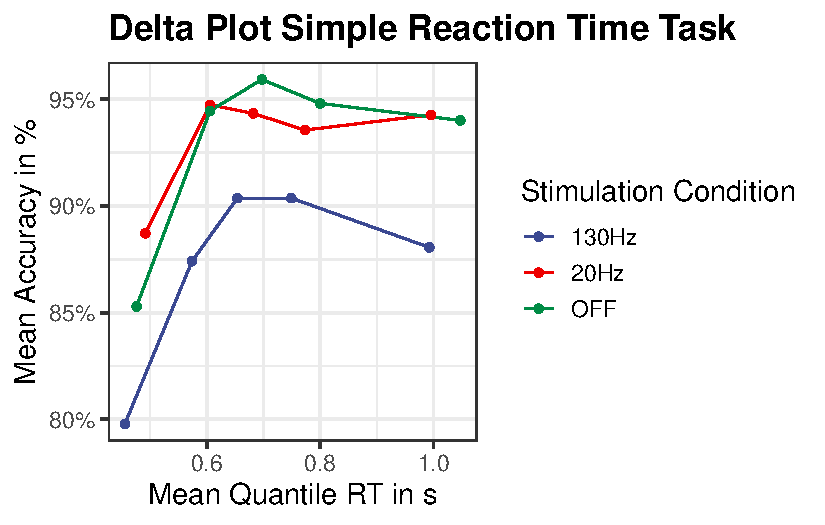
\includegraphics{MF_01_Modelfree_Analysis_files/figure-pdf/unnamed-chunk-12-1.pdf}

\hypertarget{delta-plot-flanker-task}{%
\subsubsection{Delta Plot Flanker Task}\label{delta-plot-flanker-task}}

In the flanker task, it appears that participants on 20Hz overall
responded more slowely and accurately, particulary on the incongruent
trials

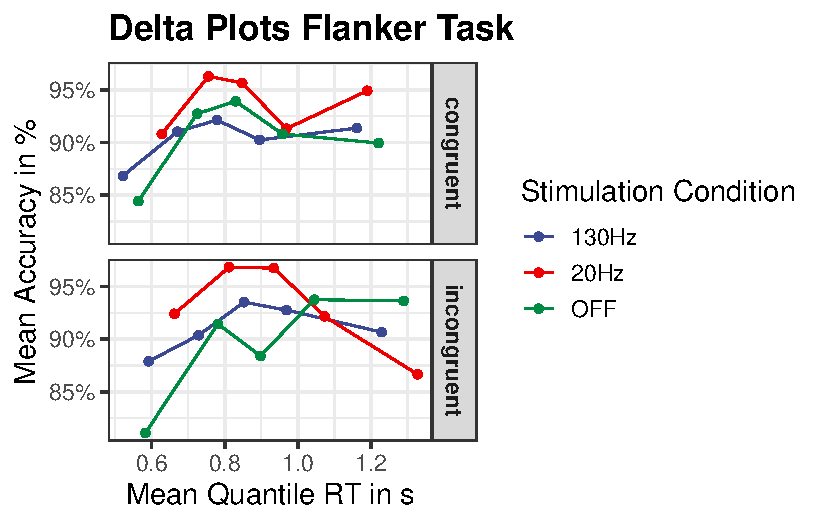
\includegraphics{MF_01_Modelfree_Analysis_files/figure-pdf/unnamed-chunk-13-1.pdf}

\hypertarget{delta-plot-go-nogo-task}{%
\subsubsection{Delta Plot Go-NoGo Task}\label{delta-plot-go-nogo-task}}

It is hard to say where participants got their competitive advantage.
They responded slightly slower and more accurately on the Go trials, but
on the Stop Go trials they responded equally fast as Off stimulation. A
parsimonious explanation would be improved cognitive control, i.e.~the
ability to override automatic response tendencies.

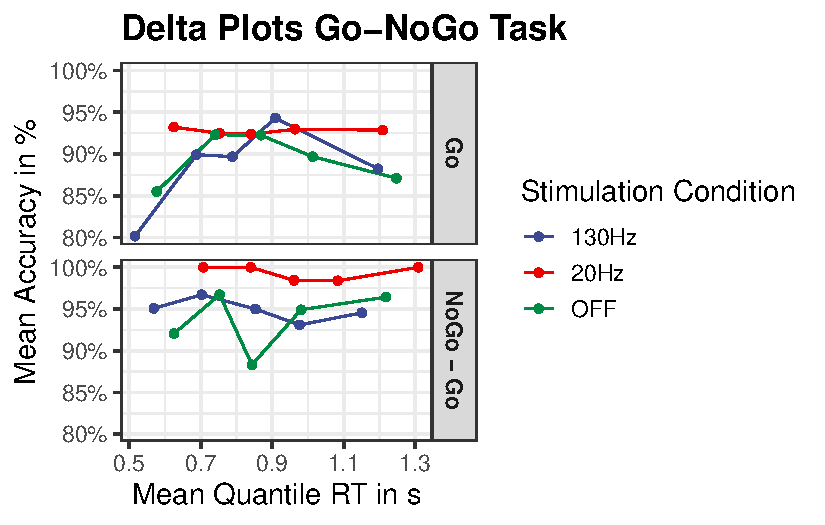
\includegraphics{MF_01_Modelfree_Analysis_files/figure-pdf/unnamed-chunk-14-1.pdf}

\hypertarget{delta-plot-stop-signal-task}{%
\subsubsection{Delta Plot Stop Signal
Task}\label{delta-plot-stop-signal-task}}

Not really much to see other than that I should exclude some trials that
are obvieously way too long

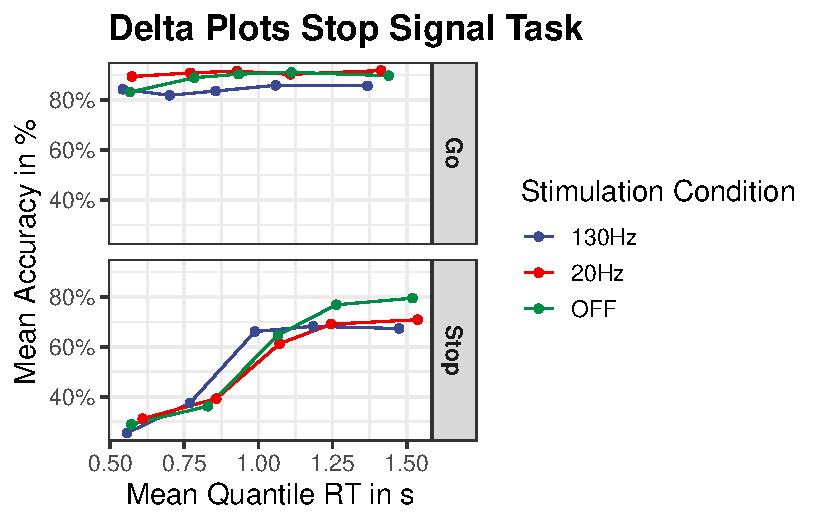
\includegraphics{MF_01_Modelfree_Analysis_files/figure-pdf/unnamed-chunk-15-1.pdf}



\end{document}
